\chapter{Towards Verifying Addition with Zero}
After realizing, that it would consume to much time to rewrite the Bitcoin-S code and even the extracted part with checkTransaction, we decided to extract the smallest unit in Bitcoin-S-Core that is worthwhile to verify.
We found the addition of two Satoshis would be a good candidate.
To make it even easier, we decided to verify only the addition of some satoshis with zero.

The initial code is this:
\lstinputlisting[language=scala]{../code/currsniporig/src/main/scala/code/initial/Code.scala}

The additions signature looks like this:
\begin{lstlisting}[language=scala]
  +(c: CurrencyUnit): CurrencyUnit
\end{lstlisting}

When we run Stainless on it, it throws the following errors:
{\footnotesize\begin{verbatim}
  [ Error  ] Code.scala:43:1: Objects cannot extend classes or implement traits,
             use a case object instead
           object Int64 extends BaseNumbers[Int64] {
           ^^^^^^^^^^^^^^^^^^^^^^^^^^^^^^^^^^^^^^^^^...
  [ Error  ] Code.scala:65:3: Stainless doesn't support abstract type members
              type A
              ^^^^^^
  [ Error  ] Code.scala:86:33: Only literal arguments are allowed for BigInt.
              def toBigInt: BigInt = BigInt(toLong)
                                            ^^^^^^
  [ Error  ] Code.scala:93:1: Objects cannot extend classes or implement traits,
             use a case object instead
            object Satoshis extends BaseNumbers[Satoshis] {
            ^^^^^^^^^^^^^^^^^^^^^^^^^^^^^^^^^^^^^^^^^^^^^^^...
  [  Info  ] Shutting down executor service.
\end{verbatim}}

So let's see how we can fix those errors.


\section{Turning object Into case object}

Stainless output:
{\footnotesize\begin{verbatim}
  [ Error  ] Code.scala:43:1: Objects cannot extend classes or implement traits,
             use a case object instead
           object Int64 extends BaseNumbers[Int64] {
           ^^^^^^^^^^^^^^^^^^^^^^^^^^^^^^^^^^^^^^^^^...
  [ Error  ] Code.scala:93:1: Objects cannot extend classes or implement traits,
            use a case object instead
            object Satoshis extends BaseNumbers[Satoshis] {
            ^^^^^^^^^^^^^^^^^^^^^^^^^^^^^^^^^^^^^^^^^^^^^^^...
\end{verbatim}}

Here, we can just change the objects from object to case object.
Stainless recommendation is to use objects for modules and case objects as algebraic data type.

This is, due to the internal design of Scala and Java.
It's possible to reason about case object but not about object.
This needs a fundamental knowledge of Scala and some functional paradigms that should not be part of this thesis.
The issue \mypound520 on Stainless GitHub gives some thoughts if you want to know more.


\section{Get Rid of Abstract Type Member}

Stainless output:
{\footnotesize\begin{verbatim}
  [ Error  ] Code.scala:65:3: Stainless doesn't support abstract type members
              type A
              ^^^^^^
\end{verbatim}}

This should be easy to rewrite by using generics instead of an abstract type, right?
Unfortunately not.
The problem is, CurrencyUnit uses one of its implementing class Satoshis.

Simplified code.
\begin{lstlisting}[language=scala]
  sealed abstract class CurrencyUnit {
    type A

    def +(c: CurrencyUnit): CurrencyUnit =
      Satoshis(satoshis.underlying + c.satoshis.underlying)

    protected def underlying: A
  }

  sealed abstract class Satoshis extends CurrencyUnit
\end{lstlisting}

What happens, if we typify CurrencyUnit with A, meaning to make it generic with type A?

Satoshis extends CurrencyUnit with type Int64, so it is of type CurrencyUnit[Int64].
That's too specific, because the addition would require CurrencyUnits of type CurrencyUnit[A] not CurrencyUnit[Int64].

Since there is no easy way to fix it and the code should stay as much as possible the original, we just remove the abstract type and fixed it to Int64.
This limits the verification a bit, but as we only want to verify the addition in satoshis, thats OK.


\section{Replace BigInt Constructor Argument With String Literal}
Stainless output:
{\footnotesize\begin{verbatim}
  [ Error  ] Code.scala:86:33: Only literal arguments are allowed for BigInt.
              def toBigInt: BigInt = BigInt(toLong)
                                            ^^^^^^
\end{verbatim}}

As described before, Stainless supports only a subset of Scala.
The BigInt from the Stainless library is a bit restricted.
It does not support dynamic BigInt construction.
Only from string literals.

Again, a simplified code version.
\begin{lstlisting}[language=scala]
  sealed abstract class Satoshis extends CurrencyUnit { 
    def toBigInt: BigInt = BigInt(toLong)
    def toLong: Long = underlying.toLong
  }
\end{lstlisting}

This would be really hard to refactor, because Bitcoin-S tries to be as much dynamic as possible so it can be used with other cryptocurrencies than bitcoins too.
Maybe it would even be impossible, because they need to parse a lot from the bitcoin network.

Luckily, we can use toBigInt on underlying directly instead of going over toLong.

After fixing all Stainless errors, a new error appears.


\section{Get Rid of Special Generics}

Stainless output:
{\footnotesize\begin{verbatim}
  [ Error  ] Code.scala:7:30: Unknown type parameter type T
             sealed abstract class Number[T <: Number[T]]
                                         ^^^^^^^^^^^^^^
\end{verbatim}}

This is a missing feature in Stainless.
To track this, there is the issue \mypound519 on GitHub.
\begin{lstlisting}[language=scala]
  sealed abstract class Number[T <: Number[T]] extends BasicArithmetic[T]  
\end{lstlisting}

For the sake of convenience we make this a concrete type by replacing T with Int64.

Now, there are two new errors.


\section{Get Rid of Concret Type}

Stainless output:
{\footnotesize\begin{verbatim}
  [Warning ] Code.scala:9:3: Could not extract tree in class: type A =
             BigInt (class scala.reflect.internal.Trees$TypeDef)
             type A = BigInt
             ^^^^^^^^^^^^^^^
\end{verbatim}}

This is easy.
We just replace all occurence of A with BigInt, since A is not overrided in an implementing class.
This is not exact the same code, because an implementing class could not override A anymore but thats fine for our verification.

This was a missing feature of Stainless that was fixed on Mai 28, 2019 with pull request \mypound470.


\section{Replace BigInt \&-Function With Bound Check}

Stainless output:
{\footnotesize\begin{verbatim}
  [ Error  ] Code.scala:22:14: Unknown call to & on result (BigInt) with arguments
             List(Number.this.andMask) of type List(BigInt)
            require((result & andMask) == result,
                    ^^^^^^^^^^^^^^^^
\end{verbatim}}

Due to the restrictions on BigInt, we can not use the \& function on.
Simplified code:
\begin{lstlisting}[language=scala]
  sealed abstract class Number extends BasicArithmetic[Int64] {
    def andMask: BigInt

    override def +(num: Int64): Int64 = apply(checkResult(underlying + num.underlying))

    private def checkResult(result: BigInt): BigInt = {
      require((result & andMask) == result, "Result was out of bounds, got: " + result)
      result
    }
  }
\end{lstlisting}

This is a bound check.
It checks, if the result of the addition is in range of the specified type, which is now the hard coded Int64.

So, we can replace the \& mask with a bound check whether the result is in range of Long.MinValue and Long.MaxValue.
Again the code gets a bit more static and it's not the exact same code anymore.

Running Stainless produces again new errors.


\section{Extracting Private Inner Classes}

Stainless output:
{\footnotesize\begin{verbatim}
  [Warning ] Code.scala:90:3: Could not extract tree in class: case private
             class SatoshisImpl extends Satoshis with Product with Serializable {
\end{verbatim}}

Stainless can not extract the private class inside the object.
Bitcoin-S uses this a lot, because they separate the class from its implementation.
Simplified:
\begin{lstlisting}[language=scala]
  object Int64 extends BaseNumbers[Int64] {
    private case class Int64Impl(underlying: BigInt) extends Int64 
  }
\end{lstlisting}

This is an easy to fix.
We just extract the private class out of the object.
This is not exactly the same code but since the class is still private it can not be extended outside of the file.

Now we get som weird warnings about require.


\section{Remove Second Parameter of require}

Stainless output:
{\footnotesize\begin{verbatim}
  [Warning ] Code.scala:51:3: Could not extract tree in class: scala.this.Predef
             .require(Int64Impl.this.underlying.>=(math.this.BigInt.long2bigInt(
             -9223372036854775808L)), "Number was too small for a int64, got: "
             .+(Int64Impl.this.underlying)) (class scala.reflect.internal.Trees$Apply)
            require(underlying >= -9223372036854775808L,
            ^^^^^^^^^^^^^^^^^^^^^^^^^^^^^^^^^^^^^^^^^^^^...
  [Warning ] Code.scala:53:3: Could not extract tree in class: scala.this.Predef
             .require(Int64Impl.this.underlying.<=(math.this.BigInt.long2bigInt(
             9223372036854775807L)), "Number was too big for a int64, got: "
             .+(Int64Impl.this.underlying)) (class scala.reflect.internal.Trees$Apply)
            require(underlying <= 9223372036854775807L,
            ^^^^^^^^^^^^^^^^^^^^^^^^^^^^^^^^^^^^^^^^^^^...
  [ Error  ] checkResult$0 depends on missing dependencies: require$1.
\end{verbatim}}

Seems like Stainless does not support the second string parameter of require or at least it throws a warning about it.
We can saftly remove it.

A new error apperas.


\section{Rewrite BigInt Comparison with Long}

Stainless output:
{\footnotesize\begin{verbatim}
  [ Error  ] inv$4 depends on missing dependencies: long2bigInt$0.
\end{verbatim}}

This error is hard to understand but we can see that there is a missing Long to BigInt conversion.
So we search for all longs in the code.
\begin{lstlisting}[language=scala]
  private case class Int64Impl(underlying: BigInt) extends Int64 {
    require(underlying >= -9223372036854775808L)
    require(underlying <= 9223372036854775807L)
  }
\end{lstlisting}

Looks like it can not compare a BigInt with a Long value.
We can easily convert this Long value to a BigInt with string literals parameter.

Finally, we get some output from Stainless about the verification in the code.
{\footnotesize\begin{verbatim}
[...]
[Warning ]  => INVALID
[Warning ] Found counter-example:
[Warning ]   thiss: { x: Object | @unchecked isNumber(x) } -> Int64Impl(0)
[Warning ]   num: { x: Object | @unchecked isInt64(x) }    -> Int64Impl(9223372036854775808)
[...]
[  Info  ] +  precond. (call checkResult(thiss, underlying(thiss) + u ...)  invalid  Code.scala:16:45
[...]
[  Info  ] total: 5  valid: 4  (4 from cache) invalid: 1  unknown: 0  time:  1.317
\end{verbatim}}

This show, that there is an invalid specification in checkResult and Stainless prints a counter example for it.

Let's ignore this for a moment and write the verification for our addition with zero.


\section{Write Specification for Verification}

As specified, our verification must only support addition with zero.
So we restrict the parameter to be zero in the precondition.
\begin{lstlisting}[language=scala]
  require(c.satoshis == Satoshis.zero)
\end{lstlisting}

We ensure the result is the same value as \emph{this} in the postcondition.
\begin{lstlisting}[language=scala]
  ensuring(res => res.satoshis == this.satoshis)
\end{lstlisting}

We can use equals (==) directly on Satoshis, because it is a case class.
The addition will now look like this:
\begin{lstlisting}[language=scala]
  override def +(c: CurrencyUnit): CurrencyUnit = {
    require(c.satoshis == Satoshis.zero)
    Satoshis(satoshis.underlying + c.satoshis.underlying)
  } ensuring(res => res.satoshis == this.satoshis)
\end{lstlisting}

That's all we need to verify our addition.

Now we will look into the previous error.


\section{Propagate require}

There is another problem with Bitcoin-S.
Bitcoin-S-Core uses require as a fail-fast method whereas Stainless needs it to verify the code.

The Stainless output again:
{\footnotesize\begin{verbatim}
  [Warning ] Found counter-example:
  [Warning ]   thiss: { x: Object | @unchecked isNumber(x) } -> Int64Impl(0)
  [Warning ]   num: { x: Object | @unchecked isInt64(x) }    -> Int64Impl(9223372036854775808)
\end{verbatim}}

Corresponding code:
\begin{lstlisting}[language=scala]
  sealed abstract class Number extends BasicArithmetic[Int64] {
    override def +(num: Int64): Int64 = apply(checkResult(underlying + num.underlying))

    private def checkResult(result: BigInt): BigInt = {
      require(
        result <= BigInt("9223372036854775807")
        && result >= BigInt("-9223372036854775808")
      )
      result
    }
  }
\end{lstlisting}

But how does Stainless find a counter example ignoring the require in checkResult?
Since Stainless is a static verification tool, it tests every possibility.
So it can use a number bigger than the maximum Int64 and pass it to the addition.
The require in checkResult fails.

Thus, we need to add the restriction from checkResult to the addition too.
\begin{lstlisting}[language=scala]
  override def +(num: Int64): Int64 = {
    require(
          num.underlying <= BigInt("9223372036854775807")
      &&  num.underlying >= BigInt("-9223372036854775808")
      && this.underlying <= BigInt("9223372036854775807")
      && this.underlying >= BigInt("-9223372036854775808")
    )
    apply(checkResult(underlying + num.underlying))
  }
\end{lstlisting}

Stainless finds another counter example:
{\footnotesize\begin{verbatim}
  [Warning ] Found counter-example:
  [Warning ]   num: { x: Object | @unchecked isInt64(x) }    -> Int64Impl(1)
  [Warning ]   thiss: { x: Object | @unchecked isNumber(x) } ->
                 Int64Impl(9223372036854775807)
\end{verbatim}}

Sure, when adding one to the maximum Int64 the require does not hold anymore.
Since we do only allow zero as a parameter the easiest way is to restrict it to zero here too.


\section{Result}

Finally, everything is green and correctly verified.
\begin{figure}[H]
	\centering
		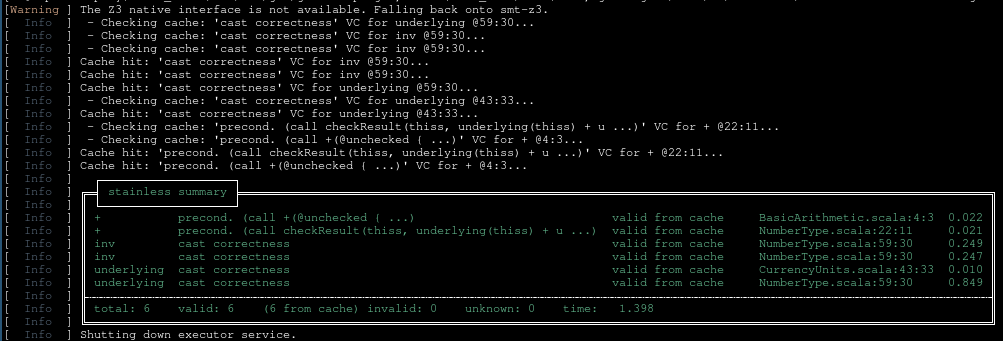
\includegraphics[scale=0.45]{images/final_verify_output.png}
	\caption{Output of Stainless verification for addition with 0 of Bitcoin-S-Cores CurrencyUnit}
	\label{fig:output1}
\end{figure}

But is it really the original code that we verified?
And why did we have to change that much?
This and other questions will be answered in the next chapter.
